\newcommand{\svcourse}{CST Part IA: Introduction to Probability}
\newcommand{\svnumber}{1}
\newcommand{\svvenue}{Churchill, Room TBD}
\newcommand{\svdate}{2022-05-14}
\newcommand{\svtime}{11:00}
\newcommand{\svuploadkey}{PO5ogKIM8KQA22FZS8IAf8gxA8XKi19jxIBVHIfFZ+3GCBXuNUXS9lVN6bNYjxM/}

\newcommand{\svrname}{Mr Matthew Ireland}
\newcommand{\jkfside}{twoside}
\newcommand{\jkfhanded}{right}

\newcommand{\studentname}{Harry Langford}
\newcommand{\studentemail}{hjel2@cam.ac.uk}


\documentclass[10pt,\jkfside,a4paper]{article}

\input{../../template/includes.tex}
% DO NOT add \usepackage commands here.  Place any custom commands
% into your SV work files.  Anything in the template directory is
% likely to be overwritten!

\usepackage{fancyhdr}

\usepackage{lastpage}       % ``n of m'' page numbering
\usepackage{lscape}         % Makes landscape easier

\usepackage{verbatim}       % Verbatim blocks
\usepackage{epsfig}         % Embed encapsulated postscript
\usepackage{array}          % Array environment
\usepackage[nolinks]{qrcode}         % QR codes
\usepackage{enumitem}       % Required by Tom Johnson's exam question header

\usepackage{hhline}         % Horizontal lines in tables
\usepackage{siunitx}        % Correct spacing of units
\usepackage{amsmath}        % American Mathematical Society
\usepackage{amssymb}        % Maths symbols
\usepackage{amsthm}         % Theorems

\usepackage{ifthen}         % Conditional processing in tex

\usepackage[top=3cm,
            bottom=3cm,
            inner=2cm,
            outer=5cm]{geometry}

% PDF metadata + URL formatting
\usepackage[
            pdfauthor={\studentname},
            pdftitle={\svcourse, SV \svnumber},
            pdfsubject={},
            pdfkeywords={9d2547b00aba40b58fa0378774f72ee6},
            pdfproducer={},
            pdfcreator={},
            hidelinks]{hyperref}

\renewcommand{\headrulewidth}{0.4pt}
\renewcommand{\footrulewidth}{0.4pt}
\fancyheadoffset[LO,LE,RO,RE]{0pt}
\fancyfootoffset[LO,LE,RO,RE]{0pt}
\pagestyle{fancy}
\fancyhead{}
\fancyhead[LO,RE]{{\bfseries \studentname}\\\studentemail}
\fancyhead[RO,LE]{{\bfseries \svcourse, SV~\svnumber}\\\svdate\ \svtime, \svvenue}
\fancyfoot{}
\fancyfoot[LO,RE]{For: \svrname}
\fancyfoot[RO,LE]{\today\hspace{1cm}\thepage\ / \pageref{LastPage}}
\fancyfoot[C]{\qrcode[height=0.8cm]{\svuploadkey}}
\setlength{\headheight}{22.55pt}

\ifthenelse{\equal{\jkfside}{oneside}}{

 \ifthenelse{\equal{\jkfhanded}{left}}{
  % 1. Left-handed marker, one-sided printing or e-marking, use oneside and...
  \evensidemargin=\oddsidemargin
  \oddsidemargin=73pt
  \setlength{\marginparwidth}{111pt}
  \setlength{\marginparsep}{-\marginparsep}
  \addtolength{\marginparsep}{-\textwidth}
  \addtolength{\marginparsep}{-\marginparwidth}
 }{
  % 2. Right-handed marker, one-sided printing or e-marking, use oneside.
  \setlength{\marginparwidth}{111pt}
 }

}{
 % 3. Alternating margins, two-sided printing, use twoside.
}

\setlength{\parindent}{0em}
\addtolength{\parskip}{1ex}

% Exam question headings, labels and sensible layout (courtesy of Tom Johnson)
\setlist{parsep=\parskip, listparindent=\parindent}
\newcommand{\examhead}[3]{\section{#1 Paper #2 Question #3}}
\newenvironment{examquestion}[3]{
    \examhead{#1}{#2}{#3}\setlist[enumerate, 1]{label=(\alph*)}\setlist[enumerate, 2]{label=(\roman*)}
    \marginpar{\qrcode{https://www.cl.cam.ac.uk/teaching/exams/pastpapers/y#1p#2q#3.pdf}}
    \marginpar{\footnotesize \url{https://www.cl.cam.ac.uk/teaching/exams/pastpapers/y#1p#2q#3.pdf}}
}{}



\usepackage{tikz}
\usepackage{listings}

\begin{document}

\begin{enumerate}

\item 

\begin{enumerate}

\item Take an initially empty hash table with five slots, with hash function $h(x) \equiv_5 x$, 
and with collisions resolved by chaining. Draw a sketch of what happens when inserting the 
following sequence of keys into it: 35, 2, 18, 6, 3, 10, 8, 5.
Hints:

You are not requested to draw the intermediate stages as separate figures, nor to show all the 
fields of each entry in detail.

Insertion into chained hash tables is simple. Hash the key, insert the key, value into the 
address which the key hashed to. If the address is occupied; then depending on implementation 
you can either traverse to the end of the linked list and then insert the key-value at the end 
of the linked list or insert the key-value into the head of the linked list. 

The expected cost of traversing to the end of the linked list is $\Theta\left(\frac{n}{\alpha}\right)$ 
where $n$ is the number of nodes in the hash table and $\alpha$ is the loading factor. I would therefore 
suggest that the standard implementation should therefore insert the key-value pair into the head of the 
list in chaining. 

Although there are cases where traversing to the end of the linked list makes more sense. For example if 
the elements put into the hash table first are more common: 
take an example from machine learning when we are storing the number of occurrences of words.

In the implementation below I insert at the head of the chain. If we were to insert at the end of the 
linked list then the order of each linked list would be reversed.

\begin{center}
\begin{tikzpicture}
\node[anchor=east] at (-0.375, 0.25) {$\equiv_5 0$};
\filldraw[draw=black, fill=lightgray!10] (-0.25, 0) rectangle (0.75, 0.5);
\filldraw[draw=black, fill=lightgray!10] (1.25, 0.02) rectangle (1.75, 0.48);
\filldraw[draw=black, fill=lightgray!10] (1.75, 0.02) rectangle (2.25, 0.48);
\filldraw[draw=black, fill=lightgray!10] (2.25, 0.02) rectangle (2.75, 0.48);
\node[anchor=center] at (2.0, 0.25) {$5$};
\draw [-stealth] (0.25, 0.25) -- (1.25, 0.25);
\draw (1.3333333333333333, 0.1) -- (1.6666666666666667, 0.4);
\filldraw[draw=black, fill=lightgray!10] (3.0, 0.02) rectangle (3.5, 0.48);
\filldraw[draw=black, fill=lightgray!10] (3.5, 0.02) rectangle (4.0, 0.48);
\filldraw[draw=black, fill=lightgray!10] (4.0, 0.02) rectangle (4.5, 0.48);
\node[anchor=center] at (3.75, 0.25) {$10$};
\draw [-stealth] (2.5, 0.19333333333333333) -- (3.0, 0.19333333333333333);
\draw [stealth-] (2.75, 0.3466666666666667) -- (3.25, 0.3466666666666667);
\filldraw[draw=black, fill=lightgray!10] (4.75, 0.02) rectangle (5.25, 0.48);
\filldraw[draw=black, fill=lightgray!10] (5.25, 0.02) rectangle (5.75, 0.48);
\filldraw[draw=black, fill=lightgray!10] (5.75, 0.02) rectangle (6.25, 0.48);
\node[anchor=center] at (5.5, 0.25) {$35$};
\draw [-stealth] (4.25, 0.19333333333333333) -- (4.75, 0.19333333333333333);
\draw [stealth-] (4.5, 0.3466666666666667) -- (5.0, 0.3466666666666667);
\draw (5.833333333333333, 0.1) -- (6.166666666666667, 0.4);
\node[anchor=east] at (-0.375, -0.25) {$\equiv_5 1$};
\filldraw[draw=black, fill=lightgray!10] (-0.25, -0.5) rectangle (0.75, 0.0);
\filldraw[draw=black, fill=lightgray!10] (1.25, -0.48) rectangle (1.75, -0.02);
\filldraw[draw=black, fill=lightgray!10] (1.75, -0.48) rectangle (2.25, -0.02);
\filldraw[draw=black, fill=lightgray!10] (2.25, -0.48) rectangle (2.75, -0.02);
\node[anchor=center] at (2.0, -0.25) {$6$};
\draw [-stealth] (0.25, -0.25) -- (1.25, -0.25);
\draw (1.3333333333333333, -0.4) -- (1.6666666666666667, -0.09999999999999998);
\draw (2.333333333333333, -0.4) -- (2.666666666666667, -0.09999999999999998);
\node[anchor=east] at (-0.375, -0.75) {$\equiv_5 2$};
\filldraw[draw=black, fill=lightgray!10] (-0.25, -1.0) rectangle (0.75, -0.5);
\filldraw[draw=black, fill=lightgray!10] (1.25, -0.98) rectangle (1.75, -0.52);
\filldraw[draw=black, fill=lightgray!10] (1.75, -0.98) rectangle (2.25, -0.52);
\filldraw[draw=black, fill=lightgray!10] (2.25, -0.98) rectangle (2.75, -0.52);
\node[anchor=center] at (2.0, -0.75) {$2$};
\draw [-stealth] (0.25, -0.75) -- (1.25, -0.75);
\draw (1.3333333333333333, -0.9) -- (1.6666666666666667, -0.6);
\draw (2.333333333333333, -0.9) -- (2.666666666666667, -0.6);
\node[anchor=east] at (-0.375, -1.25) {$\equiv_5 3$};
\filldraw[draw=black, fill=lightgray!10] (-0.25, -1.5) rectangle (0.75, -1.0);
\filldraw[draw=black, fill=lightgray!10] (1.25, -1.48) rectangle (1.75, -1.02);
\filldraw[draw=black, fill=lightgray!10] (1.75, -1.48) rectangle (2.25, -1.02);
\filldraw[draw=black, fill=lightgray!10] (2.25, -1.48) rectangle (2.75, -1.02);
\node[anchor=center] at (2.0, -1.25) {$8$};
\draw [-stealth] (0.25, -1.25) -- (1.25, -1.25);
\draw (1.3333333333333333, -1.4) -- (1.6666666666666667, -1.1);
\filldraw[draw=black, fill=lightgray!10] (3.0, -1.48) rectangle (3.5, -1.02);
\filldraw[draw=black, fill=lightgray!10] (3.5, -1.48) rectangle (4.0, -1.02);
\filldraw[draw=black, fill=lightgray!10] (4.0, -1.48) rectangle (4.5, -1.02);
\node[anchor=center] at (3.75, -1.25) {$3$};
\draw [-stealth] (2.5, -1.3066666666666666) -- (3.0, -1.3066666666666666);
\draw [stealth-] (2.75, -1.1533333333333333) -- (3.25, -1.1533333333333333);
\filldraw[draw=black, fill=lightgray!10] (4.75, -1.48) rectangle (5.25, -1.02);
\filldraw[draw=black, fill=lightgray!10] (5.25, -1.48) rectangle (5.75, -1.02);
\filldraw[draw=black, fill=lightgray!10] (5.75, -1.48) rectangle (6.25, -1.02);
\node[anchor=center] at (5.5, -1.25) {$18$};
\draw [-stealth] (4.25, -1.3066666666666666) -- (4.75, -1.3066666666666666);
\draw [stealth-] (4.5, -1.1533333333333333) -- (5.0, -1.1533333333333333);
\draw (5.833333333333333, -1.4) -- (6.166666666666667, -1.1);
\node[anchor=east] at (-0.375, -1.75) {$\equiv_5 4$};
\filldraw[draw=black, fill=lightgray!10] (-0.25, -2.0) rectangle (0.75, -1.5);
\draw (0.08333333333333333, -1.9) -- (0.4166666666666667, -1.6);
\end{tikzpicture}
\end{center}

\item Insert the same items with the following three changes: the hash table now has ten slots, 
the hash function is $h(x) = x$ mod 10, and collisions are resolved by linear probing.

\begin{center}
\begin{tikzpicture}
\node[anchor=east] at (-0.375, 0.25) {$\equiv_{10} 0$};
\filldraw[draw=black, fill=lightgray!10] (-0.25, 0) rectangle (0.75, 0.5);
\node[anchor=center] at (0.25, 0.25) {$10$};
\node[anchor=east] at (-0.375, -0.25) {$\equiv_{10} 1$};
\filldraw[draw=black, fill=lightgray!10] (-0.25, -0.5) rectangle (0.75, 0.0);
\draw (0.08333333333333333, -0.4) -- (0.4166666666666667, -0.09999999999999998);
\node[anchor=east] at (-0.375, -0.75) {$\equiv_{10} 2$};
\filldraw[draw=black, fill=lightgray!10] (-0.25, -1.0) rectangle (0.75, -0.5);
\node[anchor=center] at (0.25, -0.75) {$2$};
\node[anchor=east] at (-0.375, -1.25) {$\equiv_{10} 3$};
\filldraw[draw=black, fill=lightgray!10] (-0.25, -1.5) rectangle (0.75, -1.0);
\node[anchor=center] at (0.25, -1.25) {$3$};
\node[anchor=east] at (-0.375, -1.75) {$\equiv_{10} 4$};
\filldraw[draw=black, fill=lightgray!10] (-0.25, -2.0) rectangle (0.75, -1.5);
\draw (0.08333333333333333, -1.9) -- (0.4166666666666667, -1.6);
\node[anchor=east] at (-0.375, -2.25) {$\equiv_{10} 5$};
\filldraw[draw=black, fill=lightgray!10] (-0.25, -2.5) rectangle (0.75, -2.0);
\node[anchor=center] at (0.25, -2.25) {$35$};
\node[anchor=east] at (-0.375, -2.75) {$\equiv_{10} 6$};
\filldraw[draw=black, fill=lightgray!10] (-0.25, -3.0) rectangle (0.75, -2.5);
\node[anchor=center] at (0.25, -2.75) {$6$};
\node[anchor=east] at (-0.375, -3.25) {$\equiv_{10} 7$};
\filldraw[draw=black, fill=lightgray!10] (-0.25, -3.5) rectangle (0.75, -3.0);
\node[anchor=center] at (0.25, -3.25) {$5$};
\node[anchor=east] at (-0.375, -3.75) {$\equiv_{10} 8$};
\filldraw[draw=black, fill=lightgray!10] (-0.25, -4.0) rectangle (0.75, -3.5);
\node[anchor=center] at (0.25, -3.75) {$18$};
\node[anchor=east] at (-0.375, -4.25) {$\equiv_{10} 9$};
\filldraw[draw=black, fill=lightgray!10] (-0.25, -4.5) rectangle (0.75, -4.0);
\node[anchor=center] at (0.25, -4.25) {$8$};
\end{tikzpicture}
\end{center}


\item Imagine a hash table implementation where collisions are resolved by chaining but all the 
data stays within the slots of the original table. All entries not containing key–value pairs are 
marked with a Boolean flag and linked together into a free list.

Give clear explanations of how to implement the set(key, value) method in expected constant time, 
highlighting notable points and using high-level pseudocode where appropriate. Make use of doubly-linked 
lists if necessary.

Assume the hash table has 5 slots, is initially empty and uses the hash function $h(x) \equiv_5 x$. 
Draw five diagrams of the hash table representing the initially empty state and then the table after 
the insertion of each of the following key–value pairs: $(2, A), (2, C), (12, T), (5, Z)$. In the final 
diagram, draw all the fields and pointers of all the entries.

Every node will have a pointer to the previous element in the linked list, a pointer to the next element in a 
linked list, a boolean indicating whether it contains a key-value pair or not and if it contains a key-value 
pair then it will have elements for the key and value.

Firstly I will define ``relocating'' a key-value pair. We take a node $n$ which contains the key-value pair we 
wish to relocate. We first look at the linked list of free nodes and pop the head of this. We change it's key-value 
pair to the key-value pair we wish to relocate, copy the old nodes predecessor and successor pointer across into the 
new node and change the predecessors successor pointer and successors predecessor pointer to point to the new node. 
We then place the old node into the free list. This operation takes $\Theta(1)$ time. Note we first copy the node 
and then change pointers to cut out the old node. This ensures the chain is never severed and if the computer crashes 
mid-execution we run no risk of losing a chain of values.

To implement set(key, value) we must first hash the key and traverse to the address in the hash table 
the key hashed to. There are then 5 cases.

\begin{enumerate}[label=(\arabic*)]

\item There is no key, value in the position. In this case we change the key, value pair in the node at that position, remove 
it from the linked list of free nodes and set it's predecessor and successor pointers to itself (in my implementation all 
linked lists are circularly linked for simplicity -- it reduces the number of edge cases you need to handle at no cost).

\item There a node at that address but it was relocated. This means that no key has hashed to this address and 
so we are guaranteed there is no node with the same key as us. So we relocate the key-value which is at the address, then revert 
to case (1). Note that we relocate first so the chain in which the other address is stored is never severed.

\item There is a node at that address and it was not relocated. In this case keys have hashed to the same value as 
our key. So there is a possibility that a node with the same key as us has hashed there and is in the linked list. 
Hence, in order to ensure we do not have duplicate keys, we must search through the entire linked list to ensure no keys match our 
key: if a key matches then we should replace the value of that element and terminate. So we pass through the circularly linked list 
until either we find a node with a key that matches ours -- and replace its value. Or we reach the original location again and 
conclude that our key is not in the hash table. After that we relocate our key, value making it the second element in the linked list.

\item One of the previous cases tries to relocate a node but the free list is empty. In this case we must make a new, larger 
array and hash function, then insert every node in the old hash table into the new one then delete the old array. 
This is has a linear time complexity. However this case can only happen once every $n$ set operations. So set is amortized constant.

\end{enumerate}

\newpage

Here is a full implementation of this hash table in Java. I have commented the code as required.

\begin{lstlisting}[language=java]
import java.util.ArrayList;

public class ClosedChainHashTable<T> {

/*
initialising the required variables for the hash table. 
table stores the elements themselves (I had to use an ArrayList 
since arrays do not work with generics).
freelist is the head of the doubly linked circular list holding 
all the free elements. It needs to be doubly linked and circular 
so that we can extract from it in constant time (when inserting 
directly into an unused location via a hash).
*/
    private ArrayList<Element> table;
    private Element freelist;
    private int contains = 0;
    private int size;

    private class Element {
	
	/*
	This initialises an element into an empty element. We require 
	every element to be either free or filled. free is technically 
	unneccessary since we could check whether it held a key, value -- 
	however having a boolean to indicate this is clearer and cleaner.
	key holds the key of the node. If the node is free then key=0 
	(however this is never checked)
	value holds the payload of the element. It has arbitrary type 
	since this uses generics. If we delete the key then value is set 
	to null.
	index holds the nodes own index (a pointer to itself).
	next holds the index of the nodes successor
	previous holds the index of the nodes predecessor
	*/
        private boolean free = true;
        private int key;
        private T value;
        private final int index;
        private int previous;
        private int next;
        private boolean relocated;

        private Element(int index, int previous, int next){
            assert index >= 0;
            assert previous >= 0;
            assert next >= 0;
            this.next = next;
            this.previous = previous;
            this.index = index;
        }

        private void fill(int key, T value, int previous, int next, 
		boolean relocated){
	    /*
	    This method changes the key, value, successor 
	    and predecessor of an Element.
	    */
            if (freelist.index == index){
                freelist = table.get(freelist.next);
            }
            assert previous >= 0;
            assert next >= 0;
            table.get(this.previous).next = this.next;
            table.get(this.next).previous = this.previous;
            this.key = key;
            this.value = value;
            this.previous = previous;
            this.next = next;
            table.get(this.next).previous = index;
            table.get(this.previous).next = index;
            this.free = false;
            this.relocated = relocated;
        }

        private void clear(){
	    /*
	    This empties the node, removes it from it's 
	    linked list and adds it to the freelist.
	    */
            value = null;
            key = 0;
            this.next = freelist.index;
            this.previous = freelist.previous;
            table.get(previous).next = index;
            table.get(next).previous = index;
            relocated = false;
            free = true;
            freelist = this;
        }
    }

    public ClosedChainHashTable(int table_size){
        assert table_size >= 1;
        this.size = table_size;
        table = new ArrayList<>(size);
        Element element;
        for (int i = 0; i < size; i++) {
            element = new Element(i, (i + size - 1) % size, 
			(i + 1) % size);
            table.add(element);
        }
        freelist = table.get(0);
    }

    public void add(int key, T value) {
	/*
	First I parse the linked list for our key to avoid any 
	duplicate keys. From this point we can consider that the 
	method has ended or the key is not in the table.
	*/
	int hash_value = hash_function(key);
	Element current = table.get(hash_value);
	do {
		if (!current.free && current.key == key) {
			current.value = value;
			return;
		}
		current = table.get(current.next);
	}
	while (current.index != hash_value);

	/*
	If the hash table is full then we must resize the whole 
	table and re-insert every element. This is an expensive 
	linear time operation however it can only occur once 
	every n calls to add. So the amortized cost is constant.
	*/
        if (contains >= size) {
            size *= 2;
            ArrayList<Element> oldtable = table;
            table = new ArrayList<>(size);
            for (int i = 0; i < size; i++) {
                table.set(i, new Element(i, (i + size) % size, 
				(i + 1) % size));
            }
            for (Element element: oldtable) {
                add(element.key, element.value);
            }
        }
	/*
	Now I check the first element of the linked list. 
	If it is empty then I can fill it without issue.
	
	If it was relocated, then I should relocate it again 
	and insert my key, value into that position.
	
	If it was hashed to that address, then I should make 
	my key, value it's successor.
	*/
        int position = hash_function(key);
        Element node = table.get(position);
        if (node.free) {
            node.fill(key, value, position, position, false);
            contains++;
        }
        else if (node.relocated) {
            freelist.fill(node.key, node.value, node.previous, node.next, true);
            node.clear();
            node.fill(key, value, position, position, false);
            contains++;
        }
        else {
            freelist.fill(key, value, position, node.next, true);
            contains++;
        }
    }

    public T get(int key) {
	/*
	We hash the value and search along the linked list 
	until we return to the address the key hashed to.
	*/
        int hashvalue = hashfunction(key);
        int position = hashvalue;
        do{
            if (table.get(position).key == key){
                return table.get(position).value;
            }
            else{
                position = table.get(position).next;
            }
        }
        while (hashvalue != position);
        return null;
    }

    private int hashfunction(int k){
        return k % size;
    }


    public void delete(int key){
	/*
	If the value the key hashes to is the element we 
	wish to delete, then we must replace it with another 
	element in its linked list (if any).
	If not then we should parse through the linked list 
	until either we return to the address the key hashed 
	to or find the key. If we do find the key, we should 
	remove the node from its linked list and de-allocate 
	its key, value.
	*/
        int hash_value = hash_function(key);
        Element current = table.get(hash_value);
        if (current.free) {
            return;
        }
        if (current.key == key) {
            Element successor = table.get(current.next);
            current.value = successor.value;
            current.key = successor.key;
            current.next = successor.next;
            table.get(successor.next).previous = current.index;
            successor.clear();
            contains--;
        }
        else {
            int position = current.next;
            while (position != hash_value) {
                current = table.get(position);
                if (current.key == key) {
                    current.value = null;
                    current.key = 0;
                    table.get(current.previous).next = current.next;
                    table.get(current.next).previous = current.previous;
                    current.next = freelist.index;
                    current.previous = freelist.previous;
                    table.get(freelist.previous).next = current.index;
                    freelist.previous = current.index;
                    freelist = current;
                    contains--;
                } else {
                    position = table.get(position).next;
                }
            }
        }
    }
}
\end{lstlisting}

\end{enumerate}

In the diagram below, the pointers on the right are successor pointers, 
those on the left are predecessor pointers and a strike through the key 
or value means that no value is stored there.

\begin{center}
\begin{tikzpicture}
\node[anchor=east] at (-0.75, 0.25) {$\equiv_{5} 0$};
\node[anchor=east] at (-0.75, -0.25) {$\equiv_{5} 1$};
\node[anchor=east] at (-0.75, -0.75) {$\equiv_{5} 2$};
\node[anchor=east] at (-0.75, -1.25) {$\equiv_{5} 3$};
\node[anchor=east] at (-0.75, -1.75) {$\equiv_{5} 4$};
\draw (0, 0.5) rectangle (1, 1);
\draw (0, 0) rectangle (1, 0.5);
\draw (0, -0.5) rectangle (1, 0);
\draw (0, -1) rectangle (1, -0.5);
\draw (0, -1.5) rectangle (1, -1);
\draw (0, -2) rectangle (1, -1.5);
\draw (1, 0.5) rectangle (2, 1);
\draw (1, 0) rectangle (2, 0.5);
\draw (1, -0.5) rectangle (2, 0);
\draw (1, -1) rectangle (2, -0.5);
\draw (1, -1.5) rectangle (2, -1);
\draw (1, -2) rectangle (2, -1.5);
\node[anchor=north] at (0.5, 1) {key};
\node[anchor=north] at (1.5, 1) {value};
\draw (0.33333333333333333, 0.1) -- (0.6666666666666667, 0.4);
\draw (0.33333333333333333, -0.4) -- (0.6666666666666667, -0.1);
\draw (0.33333333333333333, -0.9) -- (0.6666666666666667, -0.6);
\draw (0.33333333333333333, -1.4) -- (0.6666666666666667, -1.1);
\draw (0.33333333333333333, -1.9) -- (0.6666666666666667, -1.6);
\draw (1.33333333333333333, 0.1) -- (1.6666666666666667, 0.4);
\draw (1.33333333333333333, -0.4) -- (1.6666666666666667, -0.1);
\draw (1.33333333333333333, -0.9) -- (1.6666666666666667, -0.6);
\draw (1.33333333333333333, -1.4) -- (1.6666666666666667, -1.1);
\draw (1.33333333333333333, -1.9) -- (1.6666666666666667, -1.6);
\draw [-stealth, black] (2, 0.25) to [loop right, out=315, in=45, looseness=1.5] (2, -0.25);
\draw [-stealth, black] (2, -0.25) to [loop right, out=315, in=45, looseness=1.5] (2, -0.75);
\draw [-stealth, black] (2, -0.75) to [loop right, out=315, in=45, looseness=1.5] (2, -1.25);
\draw [-stealth, black] (2, -1.25) to [loop right, out=315, in=45, looseness=1.5] (2, -1.75);
\draw [-stealth, black] (2, -1.75) to [loop right, out=0, in=0, looseness=1] (2, 0.25);
\draw [stealth-, black] (0, 0.25) to [loop left, out=225, in=135, looseness=1.5] (0, -0.25);
\draw [stealth-, black] (0, -0.25) to [loop left, out=225, in=135, looseness=1.5] (0, -0.75);
\draw [stealth-, black] (0, -0.75) to [loop left, out=225, in=135, looseness=1.5] (0, -1.25);
\draw [stealth-, black] (0, -1.25) to [loop left, out=225, in=135, looseness=1.5] (0, -1.75);
\draw [stealth-, black] (0, -1.75) to [loop left, out=180, in=180, looseness=1] (0, 0.25);
\end{tikzpicture}
\end{center}

Firstly we insert $2, A$. The key hashes to 2. The node at position 2 is empty -- and so we insert 
$2, A$ at position 2 and change the relevant pointers.

\begin{center}
\begin{tikzpicture}
\node[anchor=east] at (-0.75, 0.25) {$\equiv_{5} 0$};
\node[anchor=east] at (-0.75, -0.25) {$\equiv_{5} 1$};
\node[anchor=east] at (-0.75, -0.75) {$\equiv_{5} 2$};
\node[anchor=east] at (-0.75, -1.25) {$\equiv_{5} 3$};
\node[anchor=east] at (-0.75, -1.75) {$\equiv_{5} 4$};
\draw (0, 0.5) rectangle (1, 1);
\draw (0, 0) rectangle (1, 0.5);
\draw (0, -0.5) rectangle (1, 0);
\draw (0, -1) rectangle (1, -0.5);
\draw (0, -1.5) rectangle (1, -1);
\draw (0, -2) rectangle (1, -1.5);
\draw (1, 0.5) rectangle (2, 1);
\draw (1, 0) rectangle (2, 0.5);
\draw (1, -0.5) rectangle (2, 0);
\draw (1, -1) rectangle (2, -0.5);
\draw (1, -1.5) rectangle (2, -1);
\draw (1, -2) rectangle (2, -1.5);
\node[anchor=north] at (0.5, 1) {key};
\node[anchor=north] at (1.5, 1) {value};
\draw (0.33333333333333333, 0.1) -- (0.6666666666666667, 0.4);
\draw (0.33333333333333333, -0.4) -- (0.6666666666666667, -0.1);
\draw (0.33333333333333333, -1.4) -- (0.6666666666666667, -1.1);
\draw (0.33333333333333333, -1.9) -- (0.6666666666666667, -1.6);
\draw (1.33333333333333333, 0.1) -- (1.6666666666666667, 0.4);
\draw (1.33333333333333333, -0.4) -- (1.6666666666666667, -0.1);
\draw (1.33333333333333333, -1.4) -- (1.6666666666666667, -1.1);
\draw (1.33333333333333333, -1.9) -- (1.6666666666666667, -1.6);
\draw [-stealth, black] (2, 0.25) to [loop right, out=315, in=45, looseness=1.5] (2, -0.25);
\draw [-stealth, black] (2, -0.25) to [loop right, out=315, in=45, looseness=1.5] (2, -1.25);
\draw [-stealth, black, densely dashed] (2, -0.7) to [loop right, out=45, in=315, looseness=10] (2, -0.8);
\draw [-stealth, black] (2, -1.25) to [loop right, out=315, in=45, looseness=1.5] (2, -1.75);
\draw [-stealth, black] (2, -1.75) to [loop right, out=0, in=0, looseness=1] (2, 0.25);
\draw [stealth-, black] (0, 0.25) to [loop left, out=225, in=135, looseness=1.5] (0, -0.25);
\draw [stealth-, black] (0, -0.25) to [loop left, out=225, in=135, looseness=1.5] (0, -1.25);
\draw [stealth-, black, densely dashed] (0, -0.7) to [loop left, out=135, in=225, looseness=10] (0, -0.8);
\draw [stealth-, black] (0, -1.25) to [loop left, out=225, in=135, looseness=1.5] (0, -1.75);
\draw [stealth-, black] (0, -1.75) to [loop left, out=180, in=180, looseness=1] (0, 0.25);
\node [anchor=center] at (0.5, -0.75) {$2$};
\node [anchor=center] at (1.5, -0.75) {$A$};
\end{tikzpicture}
\end{center}

Next, we insert $2, C$. However, when we hash 2, we reach position 2 -- which is occupied by 
$2, A$. Note that they share a key and hash tables do not support duplicate keys. So we must 
replace $A$ with $C$. This does not involve changing any pointers.

\begin{center}
\begin{tikzpicture}
\node[anchor=east] at (-0.75, 0.25) {$\equiv_{5} 0$};
\node[anchor=east] at (-0.75, -0.25) {$\equiv_{5} 1$};
\node[anchor=east] at (-0.75, -0.75) {$\equiv_{5} 2$};
\node[anchor=east] at (-0.75, -1.25) {$\equiv_{5} 3$};
\node[anchor=east] at (-0.75, -1.75) {$\equiv_{5} 4$};
\draw (0, 0.5) rectangle (1, 1);
\draw (0, 0) rectangle (1, 0.5);
\draw (0, -0.5) rectangle (1, 0);
\draw (0, -1) rectangle (1, -0.5);
\draw (0, -1.5) rectangle (1, -1);
\draw (0, -2) rectangle (1, -1.5);
\draw (1, 0.5) rectangle (2, 1);
\draw (1, 0) rectangle (2, 0.5);
\draw (1, -0.5) rectangle (2, 0);
\draw (1, -1) rectangle (2, -0.5);
\draw (1, -1.5) rectangle (2, -1);
\draw (1, -2) rectangle (2, -1.5);
\node[anchor=north] at (0.5, 1) {key};
\node[anchor=north] at (1.5, 1) {value};
\draw (0.33333333333333333, 0.1) -- (0.6666666666666667, 0.4);
\draw (0.33333333333333333, -0.4) -- (0.6666666666666667, -0.1);
\draw (0.33333333333333333, -1.4) -- (0.6666666666666667, -1.1);
\draw (0.33333333333333333, -1.9) -- (0.6666666666666667, -1.6);
\draw (1.33333333333333333, 0.1) -- (1.6666666666666667, 0.4);
\draw (1.33333333333333333, -0.4) -- (1.6666666666666667, -0.1);
\draw (1.33333333333333333, -1.4) -- (1.6666666666666667, -1.1);
\draw (1.33333333333333333, -1.9) -- (1.6666666666666667, -1.6);
\draw [-stealth, black] (2, 0.25) to [loop right, out=315, in=45, looseness=1.5] (2, -0.25);
\draw [-stealth, black] (2, -0.25) to [loop right, out=315, in=45, looseness=1.5] (2, -1.25);
\draw [-stealth, black, densely dashed] (2, -0.7) to [loop right, out=45, in=315, looseness=10] (2, -0.8);
\draw [-stealth, black] (2, -1.25) to [loop right, out=315, in=45, looseness=1.5] (2, -1.75);
\draw [-stealth, black] (2, -1.75) to [loop right, out=0, in=0, looseness=1] (2, 0.25);
\draw [stealth-, black] (0, 0.25) to [loop left, out=225, in=135, looseness=1.5] (0, -0.25);
\draw [stealth-, black] (0, -0.25) to [loop left, out=225, in=135, looseness=1.5] (0, -1.25);
\draw [stealth-, black, densely dashed] (0, -0.7) to [loop left, out=135, in=225, looseness=10] (0, -0.8);
\draw [stealth-, black] (0, -1.25) to [loop left, out=225, in=135, looseness=1.5] (0, -1.75);
\draw [stealth-, black] (0, -1.75) to [loop left, out=180, in=180, looseness=1] (0, 0.25);
\node [anchor=center] at (0.5, -0.75) {$2$};
\node [anchor=center] at (1.5, -0.75) {$C$};
\end{tikzpicture}
\end{center}

Now we insert $12, T$. This also maps to 2. When we look, $2, C$ and $12, T$ do not have 
the same key. So we insert $T$ into the linked list following $2, C$. The 
first element in the list of free elements is at position 0. So we insert $T$ into position 
0 and change the relevant pointers.

\begin{center}
\begin{tikzpicture}
\node[anchor=east] at (-0.75, 0.25) {$\equiv_{5} 0$};
\node[anchor=east] at (-0.75, -0.25) {$\equiv_{5} 1$};
\node[anchor=east] at (-0.75, -0.75) {$\equiv_{5} 2$};
\node[anchor=east] at (-0.75, -1.25) {$\equiv_{5} 3$};
\node[anchor=east] at (-0.75, -1.75) {$\equiv_{5} 4$};
\draw (0, 0.5) rectangle (1, 1);
\draw (0, 0) rectangle (1, 0.5);
\draw (0, -0.5) rectangle (1, 0);
\draw (0, -1) rectangle (1, -0.5);
\draw (0, -1.5) rectangle (1, -1);
\draw (0, -2) rectangle (1, -1.5);
\draw (1, 0.5) rectangle (2, 1);
\draw (1, 0) rectangle (2, 0.5);
\draw (1, -0.5) rectangle (2, 0);
\draw (1, -1) rectangle (2, -0.5);
\draw (1, -1.5) rectangle (2, -1);
\draw (1, -2) rectangle (2, -1.5);
\node[anchor=north] at (0.5, 1) {key};
\node[anchor=north] at (1.5, 1) {value};
\draw (0.33333333333333333, -0.4) -- (0.6666666666666667, -0.1);
\draw (0.33333333333333333, -1.4) -- (0.6666666666666667, -1.1);
\draw (0.33333333333333333, -1.9) -- (0.6666666666666667, -1.6);
\draw (1.33333333333333333, -0.4) -- (1.6666666666666667, -0.1);
\draw (1.33333333333333333, -1.4) -- (1.6666666666666667, -1.1);
\draw (1.33333333333333333, -1.9) -- (1.6666666666666667, -1.6);
\draw [-stealth, black, densely dashed] (2, 0.25) to [loop right, out=0, in=0, looseness=1.5] (2, -0.75);
\draw [-stealth, black] (2, -0.25) to [loop right, out=315, in=45, looseness=1.5] (2, -1.25);
\draw [-stealth, black, densely dashed] (2, -0.75) to [loop right, out=45, in=315, looseness=1.5] (2, 0.25);
\draw [-stealth, black] (2, -1.25) to [loop right, out=315, in=45, looseness=1.5] (2, -1.75);
\draw [-stealth, black] (2, -1.75) to [loop right, out=0, in=0, looseness=1] (2, -0.25);
\draw [stealth-, black, densely dashed] (0, 0.25) to [loop left, out=225, in=135, looseness=1.5] (0, -0.75);
\draw [stealth-, black] (0, -0.25) to [loop left, out=225, in=135, looseness=1.5] (0, -1.25);
\draw [stealth-, black, densely dashed] (0, -0.75) to [loop left, out=180, in=180, looseness=1.5] (0, 0.25);
\draw [stealth-, black] (0, -1.25) to [loop left, out=225, in=135, looseness=1.5] (0, -1.75);
\draw [stealth-, black] (0, -1.75) to [loop left, out=180, in=180, looseness=1] (0, -0.25);
\node [anchor=center] at (0.5, -0.75) {$2$};
\node [anchor=center] at (1.5, -0.75) {$C$};
\node [anchor=center] at (0.5, 0.25) {$12$};
\node [anchor=center] at (1.5, 0.25) {$T$};
\end{tikzpicture}
\end{center}

Now we insert $5, Z$. This hashes to $0$. Position 0 is occupied by $12, T$. This was not hashed to 0 -- 
so we relocate $12, T$. The head of the free list is at position 1. So $12, T$ is relocated to 1. Now 
that the slot at 0 is free, we can insert $5, Z$ there.

\begin{center}
\begin{tikzpicture}
\node[anchor=east] at (-0.75, 0.25) {$\equiv_{5} 0$};
\node[anchor=east] at (-0.75, -0.25) {$\equiv_{5} 1$};
\node[anchor=east] at (-0.75, -0.75) {$\equiv_{5} 2$};
\node[anchor=east] at (-0.75, -1.25) {$\equiv_{5} 3$};
\node[anchor=east] at (-0.75, -1.75) {$\equiv_{5} 4$};
\draw (0, 0.5) rectangle (1, 1);
\draw (0, 0) rectangle (1, 0.5);
\draw (0, -0.5) rectangle (1, 0);
\draw (0, -1) rectangle (1, -0.5);
\draw (0, -1.5) rectangle (1, -1);
\draw (0, -2) rectangle (1, -1.5);
\draw (1, 0.5) rectangle (2, 1);
\draw (1, 0) rectangle (2, 0.5);
\draw (1, -0.5) rectangle (2, 0);
\draw (1, -1) rectangle (2, -0.5);
\draw (1, -1.5) rectangle (2, -1);
\draw (1, -2) rectangle (2, -1.5);
\node[anchor=north] at (0.5, 1) {key};
\node[anchor=north] at (1.5, 1) {value};
\draw (0.33333333333333333, -1.4) -- (0.6666666666666667, -1.1);
\draw (0.33333333333333333, -1.9) -- (0.6666666666666667, -1.6);
\draw (1.33333333333333333, -1.4) -- (1.6666666666666667, -1.1);
\draw (1.33333333333333333, -1.9) -- (1.6666666666666667, -1.6);
\draw [stealth-, black, densely dotted] (2, 0.2) to [loop right, out=315, in=45, looseness=10] (2, 0.3);
\draw [-stealth, black, densely dashed] (2, -0.25) to [loop right, out=0, in=0, looseness=2] (2, -0.75);
\draw [-stealth, black, densely dashed] (2, -0.75) to [loop right, out=45, in=315, looseness=1.5] (2, -0.25);
\draw [-stealth, black] (2, -1.25) to [loop right, out=315, in=45, looseness=1.5] (2, -1.75);
\draw [-stealth, black] (2, -1.75) to [loop right, out=0, in=0, looseness=2] (2, -1.25);
\draw [-stealth, black, densely dotted] (0, 0.2) to [loop left, out=225, in=135, looseness=10] (0, 0.3);
\draw [stealth-, black, densely dashed] (0, -0.25) to [loop left, out=225, in=135, looseness=1.5] (0, -0.75);
\draw [stealth-, black, densely dashed] (0, -0.75) to [loop left, out=180, in=180, looseness=2] (0, -0.25);
\draw [stealth-, black] (0, -1.25) to [loop left, out=225, in=135, looseness=1.5] (0, -1.75);
\draw [stealth-, black] (0, -1.75) to [loop left, out=180, in=180, looseness=2] (0, -1.25);
\node [anchor=center] at (0.5, -0.75) {$2$};
\node [anchor=center] at (1.5, -0.75) {$C$};
\node [anchor=center] at (0.5, 0.25) {$5$};
\node [anchor=center] at (1.5, 0.25) {$Z$};
\node [anchor=center] at (0.5, -0.25) {$12$};
\node [anchor=center] at (1.5, -0.25) {$T$};
\end{tikzpicture}
\end{center}

\end{enumerate}

\begin{enumerate}

\item Explain what is meant by the terms directed graph, undirected graph and bipartite 
graph.

A directed graph is a graph where edges have directions.

\begin{center}
\begin{tikzpicture}
\draw (-0.611292454541279, 1.4179190248233668) circle (0.25);
\draw (-1.7809526619153093, -0.3246130736376731) circle (0.25);
\draw (1.7221534911110759, -0.16617807196989398) circle (0.25);
\draw (-1.469756890217436, 0.2620035314256737) circle (0.25);
\draw (-0.5351752133017889, -1.0696283618768305) circle (0.25);
\draw (-1.9712390958068653, 1.849321146366571) circle (0.25);
\draw (-1.859794278233498, -1.319040224272404) circle (0.25);
\draw (1.3283496848555005, -1.420944246180687) circle (0.25);
\draw (1.168020025657777, 1.9274736433799986) circle (0.25);
\draw (0.13439728014872587, 1.6141991682667456) circle (0.25);
\draw (-1.6637943279142893, -0.10376487968058998) -- (-1.586915224218456, 0.04115533746859054);
\draw (-1.8027520382932625, -0.07556531277736678) -- (-1.9494397194289121, 1.6002733855062647);
\draw (-1.8007115211940536, -0.5738310253987827) -- (-1.8400354189547536, -1.0698222725112942);
\draw (1.4900527175544336, -0.2590717257596348) -- (-0.3030744397451465, -0.9767347080870897);
\draw (-1.586915224218456, 0.04115533746859054) -- (-1.6637943279142893, -0.10376487968058998);
\draw (-1.3261398318327886, 0.057371812132352124) -- (-0.6787922716864363, -0.864996642583509);
\draw (-1.545070323290086, 0.5003895352069601) -- (-1.8959256627342154, 1.6109351425852847);
\draw (-0.7808580549836744, -1.1158878614754377) -- (-1.6141114365516125, -1.2727807246737968);
\draw (-0.2895027750648209, -1.1159430797395484) -- (1.0826772466185326, -1.374629528317969);
\draw (-1.7517882223725758, 1.7295659203890486) -- (1.5027026176767864, -0.046422845992371384);
\draw (-1.756038561960378, -1.091587478980878) -- (-0.7150481708143989, 1.1904662795318408);
\draw (-1.8400354189547536, -1.0698222725112942) -- (-1.8007115211940536, -0.5738310253987827);
\draw (-1.6141114365516125, -1.2727807246737968) -- (-0.7808580549836744, -1.1158878614754377);
\draw (0.9180974610647725, 1.9212517700884972) -- (-1.7213165312138607, 1.8555430196580724);
\draw (0.9975086540572192, 1.7446462051906053) -- (-1.68928290663294, -1.1362127860830107);
\draw (0.9287674878463685, 1.854960036720279) -- (0.37364981796013447, 1.6867127749264652);
\draw (-0.10736768301160085, 1.5505618946915376) -- (-0.3695274913809523, 1.4815562983985748);
\draw (0.07388114240067202, 1.3716341314785503) -- (-0.474659075553735, -0.8270633250886352);
\draw (0.2259149239181208, 1.38155239549975) -- (1.2368320410861056, -1.1882974734136913);
\end{tikzpicture}
\end{center}

An undirected graph is a graph where edges do not have directions.

A bipartite graph is graph which can be divided into two disjoint groups such that 
no node in the right group can reach any other node in the right group and no node 
in the left group can reach any node in the left group.

\begin{center}
\begin{tikzpicture}
\draw (0, 4.5) circle (0.25);
\draw (0, 3.75) circle (0.25);
\draw (0, 3.0) circle (0.25);
\draw (0, 2.25) circle (0.25);
\draw (0, 1.5) circle (0.25);
\draw (0, 0.75) circle (0.25);
\draw (3, 4.125) circle (0.25);
\draw (3, 3.375) circle (0.25);
\draw (3, 2.625) circle (0.25);
\draw (3, 1.875) circle (0.25);
\draw (3, 1.125) circle (0.25);
\draw (0.211999576001272, 4.367500264999205) -- (2.788000423998728, 2.757499735000795);
\draw (0.24806946917841693, 3.7810086836473022) -- (2.751930530821583, 4.093991316352698);
\draw (0.23408229439226114, 3.662219139602902) -- (2.765917705607739, 2.712780860397098);
\draw (0.24806946917841693, 3.0310086836473022) -- (2.751930530821583, 3.3439913163526978);
\draw (0.23408229439226114, 2.912219139602902) -- (2.765917705607739, 1.962780860397098);
\draw (0.23408229439226114, 2.337780860397098) -- (2.765917705607739, 3.287219139602902);
\draw (0.211999576001272, 2.382499735000795) -- (2.788000423998728, 3.992500264999205);
\draw (0.18814417367671946, 1.6646261519671295) -- (2.8118558263232805, 3.9603738480328703);
\draw (0.16609095970747995, 0.9368523296709149) -- (2.83390904029252, 3.938147670329085);
\draw (0.24806946917841693, 0.7810086836473021) -- (2.751930530821583, 1.093991316352698);
\draw (0.211999576001272, 0.882499735000795) -- (2.788000423998728, 2.492500264999205);
\end{tikzpicture}
\end{center}

\item Given a bipartite graph, what is meant by a matching, and what is an augmenting path 
with respect to a matching?

A matching is a subset of edges in a bipartite graph which connects every node in the 
left set to zero or one nodes in the right set and every node in the right set to zero 
or one nodes in the left set.

In the below diagrams, arrows indicate direction. Dotted lines have weight 0 and full 
lines have weight 1.

\begin{center}
\begin{tikzpicture}
\draw (0, 4.5) circle (0.25);
\draw (0, 3.75) circle (0.25);
\draw (0, 3.0) circle (0.25);
\draw (0, 2.25) circle (0.25);
\draw (0, 1.5) circle (0.25);
\draw (0, 0.75) circle (0.25);
\draw (3, 4.125) circle (0.25);
\draw (3, 3.375) circle (0.25);
\draw (3, 2.625) circle (0.25);
\draw (3, 1.875) circle (0.25);
\draw (3, 1.125) circle (0.25);
\draw [dotted] (0.211999576001272, 4.367500264999205) -- (2.788000423998728, 2.757499735000795);
\draw (0.24806946917841693, 3.7810086836473022) -- (2.751930530821583, 4.093991316352698);
\draw [dotted] (0.23408229439226114, 3.662219139602902) -- (2.765917705607739, 2.712780860397098);
\draw (0.24806946917841693, 3.0310086836473022) -- (2.751930530821583, 3.3439913163526978);
\draw [dotted] (0.23408229439226114, 2.912219139602902) -- (2.765917705607739, 1.962780860397098);
\draw [dotted] (0.23408229439226114, 2.337780860397098) -- (2.765917705607739, 3.287219139602902);
\draw [dotted] (0.211999576001272, 2.382499735000795) -- (2.788000423998728, 3.992500264999205);
\draw [dotted] (0.18814417367671946, 1.6646261519671295) -- (2.8118558263232805, 3.9603738480328703);
\draw [dotted] (0.16609095970747995, 0.9368523296709149) -- (2.83390904029252, 3.938147670329085);
\draw [dotted] (0.24806946917841693, 0.7810086836473021) -- (2.751930530821583, 1.093991316352698);
\draw (0.211999576001272, 0.882499735000795) -- (2.788000423998728, 2.492500264999205);
\end{tikzpicture}
\end{center}

An augmenting path to a matching $m$ is a path in the residual graph to the 
which reaches the sink.

Let the bold arrows be the augmenting path in the residual graph formed by the matching 
above the last question.

\begin{center}
\begin{tikzpicture}
\draw (0, 4.5) circle (0.25);
\draw (0, 3.75) circle (0.25);
\draw (0, 3.0) circle (0.25);
\draw (0, 2.25) circle (0.25);
\draw (0, 1.5) circle (0.25);
\draw (0, 0.75) circle (0.25);
\draw (3, 4.125) circle (0.25);
\draw (3, 3.375) circle (0.25);
\draw (3, 2.625) circle (0.25);
\draw (3, 1.875) circle (0.25);
\draw (3, 1.125) circle (0.25);
\draw (5, 2.625) circle (0.25);
\draw (-2, 2.625) circle (0.25);
\node [anchor=center] at (5, 2.625) {$t$};
\node [anchor=center] at (-2, 2.6275) {$s$};
\draw [thin, -stealth] (-1.8176156989649788, 2.7959852822203324) -- (-0.1823843010350213, 4.329014717779668);
\draw [thin, stealth-] (-1.7821061157188627, 2.74756530990814) -- (-0.21789388428113732, 3.62743469009186);
\draw [thin, stealth-] (-1.7542819532664196, 2.6710721337625465) -- (-0.24571804673358047, 2.9539278662374535);
\draw [ultra thick, -stealth] (-1.7542819532664196, 2.5789278662374535) -- (-0.24571804673358047, 2.2960721337625465);
\draw [thin, -stealth] (-1.7821061157188627, 2.50243469009186) -- (-0.21789388428113732, 1.6225653099081399);
\draw [thin, stealth-] (-1.8176156989649788, 2.4540147177796676) -- (-0.1823843010350213, 0.9209852822203324);

\draw [thin, -stealth] (4.8, 2.775) -- (3.2, 3.975);
\draw [thin, stealth-] (4.765917705607739, 2.712780860397098) -- (3.234082294392261, 3.287219139602902);
\draw [thin, -stealth] (4.75, 2.625) -- (3.25, 2.625);
\draw [ultra thick, stealth-] (4.765917705607739, 2.537219139602902) -- (3.234082294392261, 1.962780860397098);
\draw [thin, stealth-] (4.8, 2.475) -- (3.2, 1.275);


\draw [thin, -stealth] (0.211999576001272, 4.367500264999205) -- (2.788000423998728, 2.757499735000795);
\draw [thin, stealth-] (0.24806946917841693, 3.7810086836473022) -- (2.751930530821583, 4.093991316352698);
\draw [thin, -stealth] (0.23408229439226114, 3.662219139602902) -- (2.765917705607739, 2.712780860397098);
\draw [ultra thick, stealth-] (0.24806946917841693, 3.0310086836473022) -- (2.751930530821583, 3.3439913163526978);
\draw [ultra thick, -stealth] (0.23408229439226114, 2.912219139602902) -- (2.765917705607739, 1.962780860397098);
\draw [ultra thick, -stealth] (0.23408229439226114, 2.337780860397098) -- (2.765917705607739, 3.287219139602902);
\draw [thin, -stealth] (0.211999576001272, 2.382499735000795) -- (2.788000423998728, 3.992500264999205);
\draw [thin, -stealth] (0.18814417367671946, 1.6646261519671295) -- (2.8118558263232805, 3.9603738480328703);
\draw [thin, -stealth] (0.16609095970747995, 0.9368523296709149) -- (2.83390904029252, 3.938147670329085);
\draw [thin, -stealth] (0.24806946917841693, 0.7810086836473021) -- (2.751930530821583, 1.093991316352698);
\draw [thin, stealth-] (0.211999576001272, 0.882499735000795) -- (2.788000423998728, 2.492500264999205);
\end{tikzpicture}
\end{center}

\item Prove that if no augmenting path exists for a given matching then that matching is 
maximum.

Assume there is no augmenting path. This means that the sink is not reachable 
from the source in the residual graph.

Consider the set of all nodes which are reachable from the source as a cut. The source and 
the sink are in different sets. Assume we wish to traverse from the source to the sink, 
the path we must take must cross this cut at some point. So 

The capacity of this cut is equal to the flow from all nodes in the cut to all nodes 
which are not in the cut. This is equal to the current flow of the graph. We know that the 
maximal flow is less than or equal to the capacity of any cut (where the source and sink 
are on different sides of the cut). So the maximal possible flow must be less than or equal 
to the current flow. So the current flow is equal to the maximal flow.

So the matching is maximum as required.

\item Outline an algorithm based on this property to find a maximal matching, and estimate 
its cost in terms of the number of vertices $n$ and edges $e$ of the given bipartite graph.

Relate every node in the left set to a node $s$ with an edge with capacity 1. 
Then relate every node in the right set to a node $t$ with an edge with capacity 1.
Set the capacity of all edges in the original graph to 1.
Run Ford-Fulkerson on the new graph with source $s$ and sink $t$.

When run on a graph with integral capacities, Ford-Fulkerson is guaranteed to 
result in every edge having an integral flow. Since each flow corresponds with 
two further nodes being contained in the matching, we know that the graph with the 
highest flow is isomorphic to the largest matching and Ford Fulkerson is proven to 
return the graph with the highest flow and this means the 
resultant flow graph can be converted into the largest matching.

If an edge between a node in the left graph and the right graph has flow 1 then the 
two nodes are related in the matching.

The worst-case cost of Ford-Fulkerson is $\Theta(f^*E)$ where $f^*$ is the maximal flow. 
This is because we know that for each bfs, Ford-Fulkerson will augment the flow by an 
integral amount (on graphs where the flow is integral). This means that there are 
at worst $f^* + 1$ bfs's. The complexity of a bfs is $\Theta(V + E)$. However, when we 
run Ford-Fulkerson, we know that the graph is connected meaning that, $\Theta(V) \in O(E)$ 
and so the complexity is $\Theta(f^*E)$.

Note that in a matching with $V$ vertices, the highest possible flow rate ($f^*_{\max}$) is $\frac{V}{2}$ 
and occurs when every vertex is involved in the matching. So the worst case of ford-fulkerson 
on a matching is $\Theta(VE)$.

In this graph there are $n$ nodes and $e$ edges: so the worst-case complexity of this 
algorithm is $\Theta(ne)$.

\end{enumerate}

\end{document}